\chapter{Evaluation}
\label{ch:evaluation}
\section{Criteria of Assessment}
For evaluation of this project, we consider our aims and objectives as discussed in the introduction, amongst other considerations from . Deriving from these objectives, we can determine a set of criteria that we can base our evaluation upon:

\begin{enumerate}[label = {}, leftmargin=\widthof{Relevancy |}+\labelsep]
    \item[Accuracy |] The system is capable of producing accurate outputs for the stoichiometries and precursors that a user may desire.
    
    \item[Relevancy |] The system produces results that are suitably relevant to the user without too many “garbage” results, or at least orders results by relevance.

\item[Speed |] The system returns its results in a reasonable amount of time.
\end{enumerate}

\subsection{Accuracy}
In the interests of evaluating accuracy, we took known, pre-existing stoichiometries and precursor calculations from publicly available sources and used them to ensure that the program was calculating its outputs correctly. By taking a suitably sized collection of pre-calculated values, we repeatedly tested the system using inputs designed to acquire these values, using any failed cases to re-evaluate what went wrong and adjust the system accordingly. 

After more thorough testing of a multitude of precursor and stoich combinations, we have concluded that the program is accurate to a suitable degree in most cases. As mentioned previously in the design section, we did remove uncommon charge balances from the calculation in the interest of avoiding untenable combinations as implemented in our current release, so some possible stoichiometries will not be generated. Nevertheless, the outputs the system does generate are in general perfectly viable and correct, and functionality for the rarer charges may be added in future releases.

\subsection{Relevancy}
The system produces a range of stoichiometries based on the user input, presented in a list. As the user goes down this list, the size and composition of these stoichiometries becomes increasingly excessive and unwieldy, and for the most part we expect that only a small selection of optimal results would ever be used by the end user, with the other results only being used in the interests of further analysis and pure curiosity.

By giving the user control of the scope of the results returned to them, both in terms of the maximum mass of the given stoichiometries and the maximum number of results generated, the user can refine their search such that while the system calculates (or retrieves from the database) many potential results, it will only display those results that fit the user’s defined criteria. As such, the user can tailor the relevancy of the results to their liking. In addition, by ranking the results based according to our defined criteria of suitability and displaying them in that order, we ensure that the first few results in the list are likely the most desirable and relevant to the user.

In summary, the program maintains relevant results by empowering the user to more strictly control the results they receive, while allowing them to view the full data set if they so desire. The results produced nearer the top of the list are, in general, the smallest possible stoichiometries form-able from the selected precursors, though in some cases stoichiometries are generated without every desired precursor included. This is minimal issue, however, since enough data is generated that a user can simply ignore these and pick out the stoichiometries that fulfil their needs exactly.

\subsection{Speed}
In earlier versions of the program, the calculator speed varied greatly, with certain calculations taking an unreasonably long time. Given that a user may become impatient if they are made to wait for even a simple stoichiometry calculation, a number of approaches were considered to address the issue. Initially, we considered simply including a loading screen when the user requests a calculation to reassure the user that the system is working, but a more intuitive solution was sought to actually cut down the runtime.

In our original implementation, the calculators used a method whereby they calculated every possible combination of elements - with each element proportion measured as a real number from 0 to 1, the program would incrementally run through the combinations in very small margins (approx. 10-3). The program would then need to evaluate and 

The resultant cache file generated by calculations under this method ranged in size between 30 to 100 megabytes, which is unacceptable for common use. The speed of the system was equally unacceptable - Analysis of the runtime on a function-by-function basis revealed that almost half of the runtime was being taken up by generating weights for each stoichiometry and by validation checks. In  Attempts at optimisation of this method could only result in an approximately 33\% increase in program speed.

In our final implementation, we adjusted the system to run on a much smaller set of real numbers, tying the number generated to the number of results requested by the user. In this method, we generate only as many results as the user wants rather than generating every possible result and then checking to see which of them fits the user criteria.

For a user requesting 1000 samples, the new method generates only 34 numbers to run evaluation on where the previous method would generate over 104 numbers, which results in far less validation runs being needed. As to the overall speed, in a set of tests utilizing the same amount of precursors and stoichiometries, the original method completed computation in approx. 2.67 seconds, while the final method completed in just over 0.02 seconds, representing an approx. $13,330\%$ increase in speed. This significant improvement was accepted as more than sufficient for our needs.

\subsection{Test Cases}
\subsubsection{Test 1}
\begin{enumerate}[label = {}, leftmargin=\widthof{Precursor Selection |}+\labelsep]
    \item[Input selection |] $Li_{17}AlSi_{4}S_{16}C_{l4}$
    \item[Precursor Selection |] $LiCl$ $Li_2S$ $Al_2S_3$ $Si$ $S$
    \item[Samples requested |] 1000
    \item[Target mass |] 250mg
    \item[Execution Time |] 0.02006396s (5 run average, wall clock)
\end{enumerate}

\begin{table}[h!]
    \centering
    \begin{tabular}{@{}ccccc@{}}
        \toprule
        \multicolumn{5}{c}{Expected Mass}              \\ \midrule
        $LiCl$ & $Li_2S$ & $Al_2S_3$ & $Si$   & $S$    \\
        46.5mg & 81.8mg  & 20.6mg    & 30.8mg & 70.3mg \\ \bottomrule
    \end{tabular}
\end{table}

\begin{table}[h!]
    \centering
    \begin{tabular}{@{}ccccc@{}}
        \toprule
        \multicolumn{5}{c}{Computed Mass}                        \\ \midrule
        $LiCl$    & $Li_2S$   & $Al_2S_3$ & $Si$      & $S$      \\
        46.4787mg & 81.9083mg & 20.5671mg & 30.7729mg & 70.273mg \\ \bottomrule
    \end{tabular}
\end{table}

\subsubsection{Test 2}
\begin{enumerate}[label = {}, leftmargin=\widthof{Precursor Selection |}+\labelsep]
    \item[Input selection |] $Li_{10}Al_2SiS_8Cl_4$
    \item[Precursor Selection |] $Li_2S$ $AlCl_3$ $Al_2S_3$ $Si$ $S$
    \item[Samples requested |] 1000
    \item[Target mass |] 250mg
    \item[Execution Time |] 0.03052124s (5 run average, wall clock)
\end{enumerate}

\begin{table}[h!]
\centering
\begin{tabular}{@{}ccccc@{}}
\toprule
\multicolumn{5}{c}{Expected Mass} \\ \midrule
$Li_2S$ & $AlCl_3$ & $Al_2S_3$ & $Si$ & $S$ \\
104.5mg & 22.8mg & 80.8mg & 12.8mg & 29.1mg \\ \bottomrule
\end{tabular}
\end{table}

\begin{table}[h!]
\centering
\begin{tabular}{@{}ccccc@{}}
\toprule
\multicolumn{5}{c}{Computed Mass} \\ \midrule
$Li_2S$ & $AlCl_3$ & $Al_2S_3$ & $Si$ & $S$ \\
104.538mg & 22.7495mg & 80.7996mg & 12.7643mg & 29.1486mg \\ \bottomrule
\end{tabular}
\end{table}

\subsubsection{Test 3}
\begin{enumerate}[label = {}, leftmargin=\widthof{Precursor Selection |}+\labelsep]
    \item[Input selection |] $LiAlSO$
    \item[Precursor Selection |] $Li_2S$ $Al_2S_3$ $Al_2O_3$ $LiAlO_2$ $Li_2O$
    \item[Samples requested |] 1000
    \item[Target mass |] 500mg
    \item[Execution Time |] 0.02132445s (5 run average, wall clock)
\end{enumerate}

\begin{table}[h!]
\centering
\begin{tabular}{@{}ccccc@{}}
\toprule
\multicolumn{5}{c}{Expected Mass} \\ \midrule
$Li_2S$ & $Al_2S_3$ & $Al_2O_3$ & $LiAlO_2$ & $Li_2O$ \\
0mg & 30.53mg & 0mg & 13.40mg & 6.07mg \\ \bottomrule
\end{tabular}
\end{table}

\begin{table}[h!]
\centering
\begin{tabular}{@{}ccccc@{}}
\toprule
\multicolumn{5}{c}{Calcualted Mass} \\ \midrule
$Li_2S$ & $Al_2S_3$ & $Al_2O_3$ & $LiAlO_2$ & $Li_2O$ \\
0mg & 30.5155mg & 0mg & 13.4014mg & 6.08305mg \\ \bottomrule
\end{tabular}
\end{table}

\subsection{Strengths and Weaknesses}
To summarise the strengths and weaknesses of our project, we consider the qualities discussed above as well as several other elements discussed in the design and implementation phase.

Strengths:
\begin{enumerate}
    \item The results produced by the project are accurate and viable solutions that a chemist can use in a lab setting.
    
    \item The user is given control of the scope and size of the samples returned so that they can return a simple list if they are just looking for a solution, or a more exhaustive list if they wish to study the output for educational purposes.
    
    \item Calculator runs in less than a second on a single thread
    
    \item The system is designed to be remotely accessible, so that a user only needs to access the web server page to use the system from anywhere on the network (although it is possible to set up a local version if so desired).
    
    \item The system is designed to be modular in nature with components being easy to add and remove without much conflict.
\end{enumerate}

Weaknesses:
\begin{enumerate}
    \item No support currently for automatic generation of rarer charge states of elements in precursors, though the user can manually input custom precursors if they wish.
    
    \item Login system not implemented due to time constraints, currently anyone can access the system with any login code, though the system remains remotely accessible.
    
    \item No currently implemented parallelism makes it scale poorly with higher dimensions (nr of precursors).
\end{enumerate}

\subsection{Involvement of MIF Staff}
As previously specified, we worked closely with personnel employed within the Materials Innovation Factory (who commissioned the development of the system) to continually evaluate progress on the project and to provide feedback and further ideas for development. We scheduled frequent meetings with our supervisors as well as other members in order to receive an outside view of our work. Doing so helped to identify issues with the program that had escaped our notice, in terms of both interface design and the accuracy and suitability of outputs.

To reiterate further, as those we worked with were part of the project development, we do not consider them 3rd party evaluators. Meetings and evaluations were all conducted within the bounds of the MIF and staff actively involved in the commission of the project.

\section{Performance Data}
\begin{figure}[h!]
    \centering
    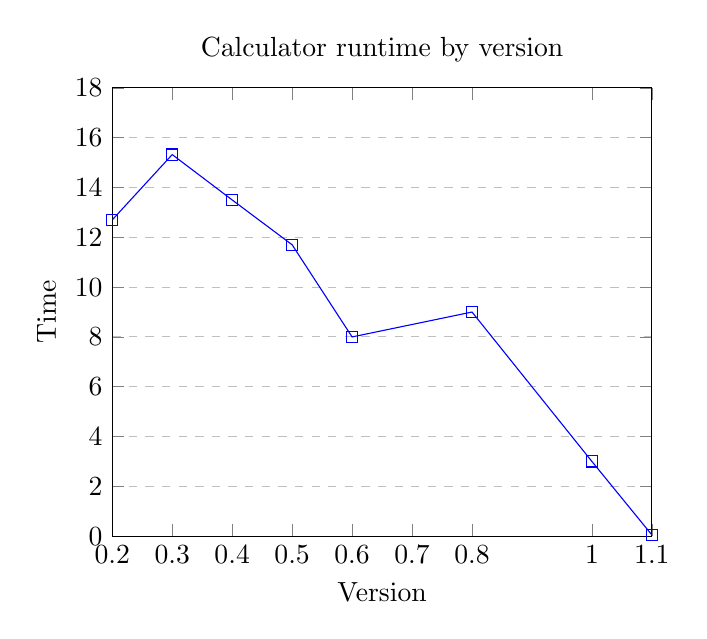
\begin{tikzpicture}
        \begin{axis}[
            title={Calculator runtime by version},
            xlabel={Version},
            ylabel={Time},
            xmin=0.2, xmax=1.1,
            ymin=0, ymax=18,
            xtick={0.2, 0.3, 0.4,0.5,0.6,0.7,0.8,1.0,1.1},
            ytick={0,2,4,6,8,10,12,14,16,18},
            legend pos=north west,
            ymajorgrids=true,
            grid style=dashed,
        ]
         
        \addplot[
            color=blue,
            mark=square,
            ]
            coordinates {
            (0.2,12.7)(0.3,15.322)(0.4, 13.5)(0.5, 11.7)(0.6, 8)(0.8, 9)(1.0, 3)(1.1,0.05)
            };
         
        \end{axis}
    \end{tikzpicture}
    \label{fig:runtime}
\end{figure}
